%# -*- coding: utf-8-unix -*-
%%==================================================
%% chapter01.tex for SJTU Master Thesis
%%==================================================

%\bibliographystyle{sjtu2}%[此处用于每章都生产参考文献]
\chapter{相关工作}
\label{chap:Work}
除了前几章介绍的主要工作意外,我们还使用AKI-最小割算法\ref{alg:AKI}对其他轻量级密码函数进行了分析。
在介绍这些轻量级分组密码的AKI结果之前,需要注意以下两点:
\begin{enumerate}
    \item 所有$r$轮的计算路径/密钥依赖路径均由一个比特产生,即,我们会使用部分明文和轮密钥来进行部分加密,最终得到一个比特的值。
        对于攻击者,最坏的情况无非是需要使用所有密钥依赖路径上的轮密钥比特来得到想计算的这一比特,因此对于设计者来说,如果该路径的AKI达到理论最大值即是最佳的情况。
    \item 所有$r$轮的路径均为前向路径,即从该比特向前推断依赖关系,以得到一条加密方向所需比特的路径。解密方向的路径同样可以由解密时的依赖矩阵得到,由于工作类似我们不再赘述。
\end{enumerate}

\section{PRESENT和RECTANGLE}
PRESENT\citen{Bogdanov}和RECTANGLE\citen{zhang2015rectangle}是相类似的两种SPN结构的面向比特的轻量级分组密码。
PRESENT由31轮加密组成,而RECTANGLE由25轮加密组成。
两者的分组长度均为64,而主密钥长度均支持80比特和128比特两个版本。

\textbf{PRESENT的密钥编排方案:}
PRESENT-80的80比特主密钥被存储在一个密钥寄存器中,可以被表示为$K_0=k_{79}k_{78}\dots k_0$。
第$i$轮的64比特轮密钥将提取密钥寄存器中的最左侧64比特,即$RK_i=\kappa_{63}\kappa_{62}\dots\kappa_{0}=k_{79}k_{78}\dots k_{16}$。
每经过一轮,密钥寄存器将会经过如下改变:
\begin{enumerate}
    \item $[k_{79}k_{78}\dots k_1k_0]=[k_{18}k_{17}\dots k_{20}k_{19}]$
    \item $[k_{79}k_{78}k_{77}k_{76}]=S[k_{79}k_{78}k_{77}k_{76}]$
    \item $[k_{19}k_{18}k_{17}k_{16}k_{15}]=[k_{19}k_{18}k_{17}k_{16}k_{15}]\oplus\mbox{round\_counter}$
\end{enumerate}

在PRESENT-128版本中,$RK_i=\kappa_{63}\kappa_{62}\dots\kappa_{0}=k_{127}k_{126}\dots k_{64}$
而密钥寄存器更新方式如下:
\begin{enumerate}
    \item $[k_{127}k_{126}\dots k_1k_0]=[k_{66}k_{65}\dots k_{68}k_{67}]$
    \item $[k_{127}k_{126}k_{125}k_{124}]=S[k_{127}k_{126}k_{125}k_{124}]$
    \item $[k_{123}k_{122}k_{121}k_{120}]=S[k_{123}k_{122}k_{121}k_{120}]$
    \item $[k_{66}k_{65}k_{64}k_{63}k_{62}]=[k_{66}k_{65}k_{64}k_{63}k_{62}]\oplus\mbox{round\_counter}$
\end{enumerate}

\textbf{RECTANGLE的密钥编排方案:}
RECTANGLE-80的主密钥被存在一个$5\times 16$的矩阵中,见图\ref{fig:Rec80}。
\begin{figure}[htbp]
    \centering
$\begin{bmatrix}
v_{15}&\ldots& v_2&v_1&v_0\\
v_{31}&\ldots& v_{18}&v_{17}&v_{16}\\
v_{47}&\ldots& v_{34}&v_{33}&v_{32}\\
v_{63}&\ldots& v_{50}&v_{49}&v_{48}\\
v_{79}&\ldots& v_{66}&v_{65}&v_{64}\\
\end{bmatrix}$ \quad \quad
$\begin{bmatrix}
\k_{0,15}&\ldots& \k_{0,2}&\k_{0,1}&\k_{0,0}\\
\k_{1,15}&\ldots& \k_{1,2}&\k_{1,1}&\k_{1,0}\\
\k_{2,15}&\ldots& \k_{2,2}&\k_{2,1}&\k_{2,0}\\
\k_{3,15}&\ldots& \k_{3,2}&\k_{3,1}&\k_{3,0}\\
\k_{4,15}&\ldots& \k_{3,2}&\k_{3,1}&\k_{3,0}\\
\end{bmatrix}$
\bicaption[fig:Rec80]{RECTANGLE-80的密钥矩阵}{RECTANGLE-80的80比特密钥的二维表示方法}{Key Matrix}{An 80-bit key state of RECTANGLE and its two-dimensional representation.}
\end{figure}
令$Row_i=\k_{i,15}||\cdots||\k_{i,1}||\k_{i,0}$为密钥矩阵的第$i$行,$0\leq i\leq 4$。
$Row_i$可以被看做是一个16比特的字。
加密过程中,每一轮的轮密钥$RK_i$包含了密钥矩阵的前4行,即$RK_i=Row_3||Row_2||Row_1||Row_0$。
提取出轮密钥后,密钥寄存器将会进行如下变换:
\begin{enumerate}
    \item $k'_{3,j}||k'_{2,j}||k'_{1,j}||k'_{0,j}=S(k_{3,j}||k_{2,j}||k_{1,j}||k_{0,j})$,$j=0,1,2,3$。
    \item 对密钥寄存器进行一个类1轮Feistel结构的变换:
        $$\begin{array}{ccc}
            Row'_0=(Row_0\ll 8)\oplus Row_1, & Row'_1=Row_2, & Row'_2=Row_3\\
            Row'_3=(Row_3\ll 12)\oplus Row_4, & Row'_4=Row_0. & 
        \end{array}$$
    \item $k'_{0,4}||k'_{0,3}||k'_{0,2}||k'_{0,1}||k'_{0,0}=(k_{0,4}||k_{0,3}||k_{0,2}||k_{0,1}||k_{0,0})\oplus RC[i]$
\end{enumerate}

RCTANGLE-128已经在第\ref{chap:App}章中简要介绍过了,在此不再赘述。

\textbf{例:}在RECTANGLE-80中,对于一个由$X_3^0$向前推出的计算路径(见图\ref{fig:3KDP}),其密钥依赖路径为:
\begin{center}
    \noindent
    \footnotesize{$k_0\hat{}[0,2$-$4,6$-$8,14$-$16,18$-$20,22$-$24,30$-$31,34$-$36,38$-$40,46$-$48,50$-$52,54$-$56,62,63]$}

  \noindent
  \centering
  \footnotesize{$\rightarrow k_1\hat{}[0,3,4,15,16,19,20,31,32,35,36,47,48,51,52,63]\rightarrow k_2\hat{}[0,16,32,48]$.}
  \end{center}
但是其AKI仅为42比特,其中$k_1\hat{}[0,15,16,19,20,31,32,35,36,47]$, $k_2\hat{}[0,16,32,48]$为冗余密钥。
\begin{figure}[htbp]
    \centering
    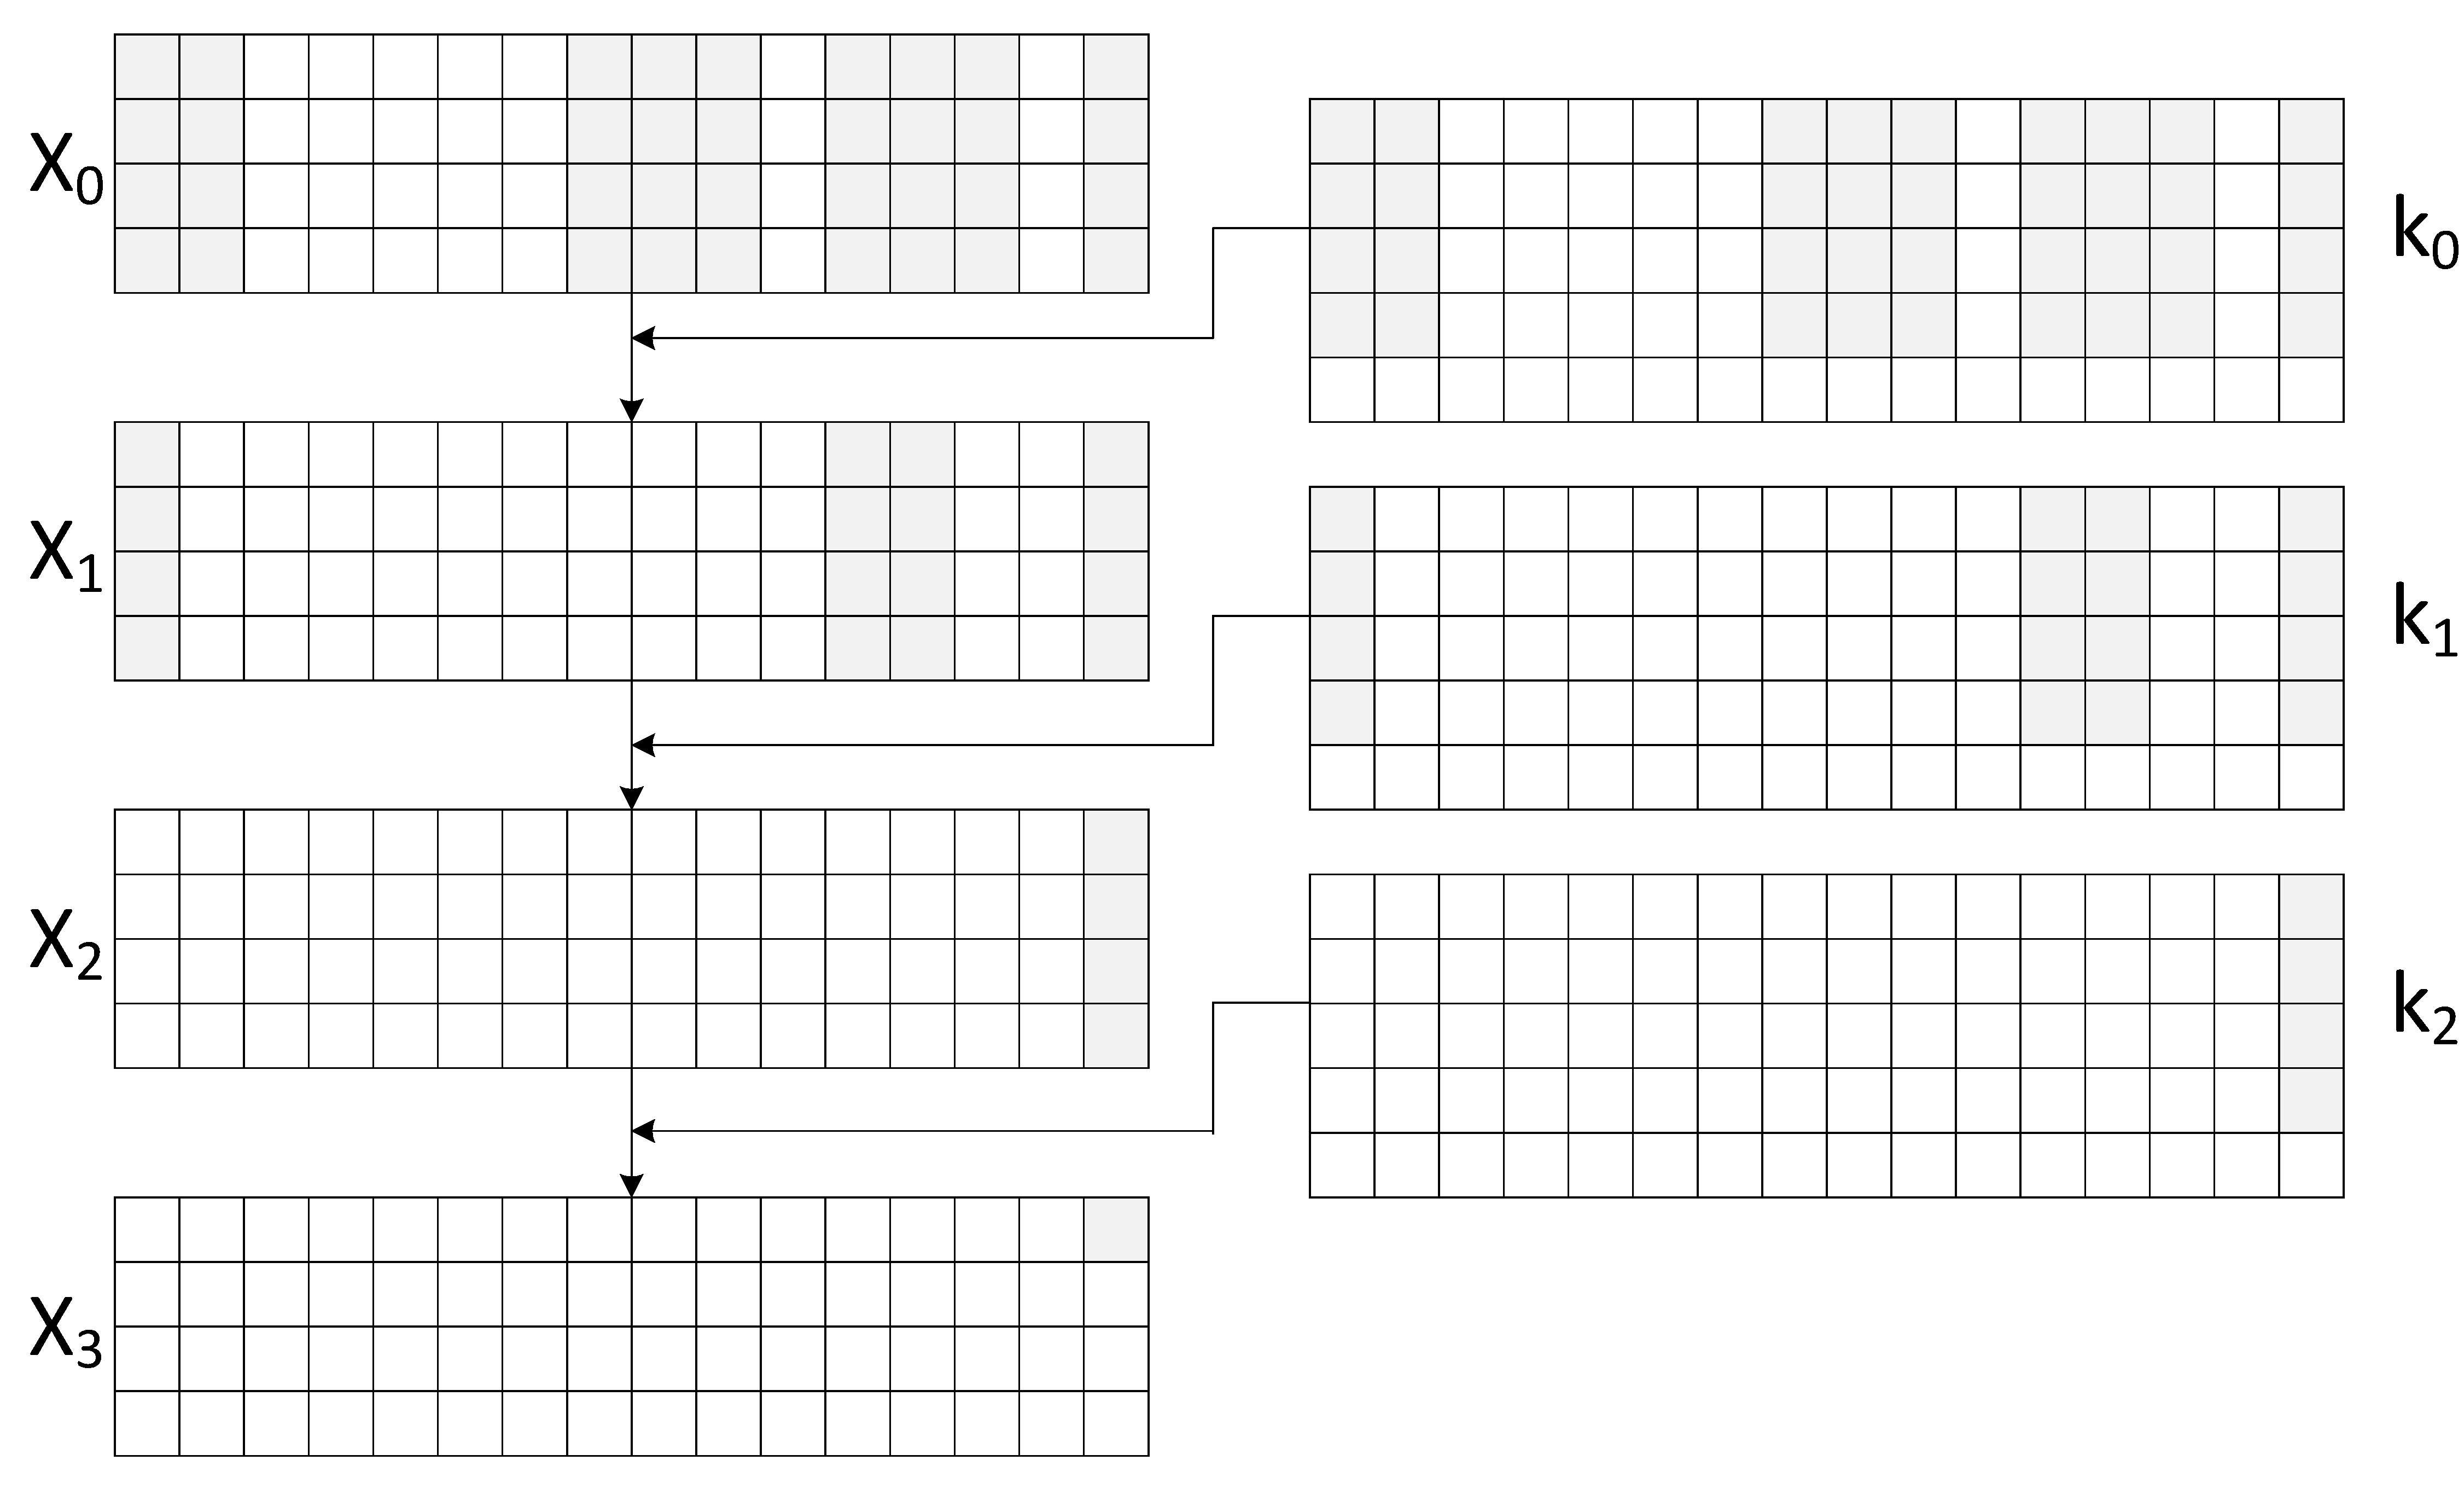
\includegraphics[height=5.5cm]{3KDP}
    \bicaption[fig:3KDP]{RECTANGLE-80的一条3轮路径}{RECTANGLE-80的一条3轮的计算路径和其密钥依赖路径}{3-round KDP}{A 3-round CP and KDP of RECTANGLE-80}
\end{figure}

由于PRESENT和RECTANGLE的结构、主密钥和分组长度都十分相似,在RECTANGLE的设计文档\citen{zhang2015rectangle}中作者比较了这两种加密方式的效率和安全性。
经过对以上4种密钥编排方案的AKI计算(见表\ref{tab:PREREC}),我们发现即使RECTANGLE的轮函数由于使用了bit-slice技术且仔细挑选了S盒而拥有更高的安全性和效率,但是它的AKI却在同轮比PRESENT少。
因此我们认为,PRESENT的密钥编排方案更加“配合”它的轮函数。

\begin{table}[tbp]
\centering
\begin{tabular}{c|cc|cc|cc|cc}
\hline
&\multicolumn{2}{c|}{RECTANGLE-80\quad}&\multicolumn{2}{c|}{PRESENT-80}&\multicolumn{2}{c|}{RECTANGLE-128\quad}&\multicolumn{2}{c}{PRESENT-128}\\
\hline
&$TKI$&\quad $AKI$&$TKI$&\quad $AKI$&$TKI$&\quad $AKI$&$TKI$&\quad $AKI$\\
$r=1$&4&4&4&4&4&4&4&4\\
$r=2$&20 & \textcolor{red}{18}&20 &20&20& \textcolor{red}{18}  &20 &20\\
$r=3$&56 &\textcolor{red}{42} &80 &\textcolor{red}{64}&56 &\textcolor{red}{44}  &84 &\textcolor{red}{77}\\
$r=4$&80 &\textcolor{red}{73} &80 &\textbf{80}&120 &\textcolor{red}{83} &128 &\textcolor{red}{125}\\
$r=5$&80 &\textbf{80}         &-  &-          &128 &\textcolor{red}{103} &128 &\textbf{128}\\
$r=6$&-&-&-&-&128 &\textcolor{red}{120}&- &-\\
$r=7$&-&-&-&-&128 &\textbf{128} &- &-\\
\hline
\end{tabular}
\bicaption[tab:PREREC]{PRESENT和RECTANGLE的AKI}{PRESENT-80/128和RECTANGLE-80/128的AKI}{AKI}{AKI of PRESENT and RECTANGLE}
\end{table}

另外,Zhang等人在设计RECTANGLE\citen{zhang2015rectangle}时单独分析了RECTANGLE的密钥编排方案(没有考虑轮函数),并称其80比特版本中,任意连续两轮的子密钥均依赖于所有80比特主密钥。
但是在结合轮函数和密钥编排方案两者的扩散程度的分析后我们发现,任意2,3,4轮的密钥依赖路径均没有完全包含整个密钥空间(密钥信息不足80比特),直到第5轮才得到完全的扩散。
类似地,在128比特版本中,作者称任意连续4轮子密钥均依赖于所有128比特子密钥,而在我们的结果中RECTANGLE-128使用了7轮才将密钥依赖路径扩散到整个密钥空间。

导致以上密钥信息泄露的其中一个主要的原因是密钥编排方案和轮函数两者扩散时的重叠。
这提醒了我们轮函数与密钥编排方案的扩散方式应该相辅相成,不能两者单独考虑。

\section{Midori和LED}
Midori是Banik等人\citen{banik2014midori}在2015年亚密会上提出的一种低能耗的轻量级SPN结构的分组密码。
Midori提供了两种不同的分组长度,分别为Midori-64(拥有64比特的分组长度)和Midori-128(128比特的分组长度)。
主密钥长度均为128比特。

Midori-64中,128比特的主密钥$K$被分为两个64比特的密钥$K_0$和$K_1$,即$K=K_0||K_1$。
白化密钥$WK=K_0\oplus K_1$,轮密钥$RK_i=K_{i\mbox{ mod }2}\oplus\alpha_i$,$0\leq i\leq 14$。
Midori-128中,白化密钥$WK=K$,轮密钥$RK_j=K\oplus\alpha_j$,$0\leq j\leq 18$。
其中$\alpha_i$是轮常数。

LED是由Guo等人\citen{Guo2011}在2011年提出的一个类AES的轻量级分组密码。
其分组长度为64比特,主密钥长度支持64比特和128比特。
LED的密钥编排方案十分简单,甚至可以说没有密钥编排方案——对于64比特长度的主密钥,$RK_i=K$,即轮密钥即为主密钥;
而对于128比特长度的主密钥,主密钥将会被分为两部分$K_0$和$K_1$,在加密时轮流使用$K_0$和$K_1$。

类似PRESENT和RECTANGLE,我们对LED和Midori计算了前几轮所有的密钥依赖路径的AKI,相关结果总结在

\begin{table}[htbp]
\centering
\begin{tabular}{c|cc|cc|cc|cc}
\hline
&\multicolumn{2}{c|}{Midori-64\quad}&\multicolumn{2}{c|}{Midori-128}&\multicolumn{2}{c|}{LED-64\quad}&\multicolumn{2}{c}{LED-128}\\
\hline
&$TKI$&\quad $AKI$&$TKI$&\quad $AKI$&$TKI$&\quad $AKI$&$TKI$&\quad $AKI$\\
$r=1$&25&\textcolor{red}{24}&13&\textcolor{red}{12}&64&64&64&64\\
$r=2$&85 &\textcolor{red}{72}&77 &\textcolor{red}{60}&64& \textbf{64}  &128 &\textbf{128}\\
$r=3$&128 &\textbf{128} &128 &\textcolor{red}{124}&- &- &- &-\\
$r=4$&- &- &128 &\textbf{128}&- &- &- &-\\
\hline
\end{tabular}
\bicaption[tab:MidoriLED]{Midori和LED的AKI}{Midori-64/128和LED-64/128的AKI}{AKI}{AKI of Midori and LED}
\end{table}

Midori和LED的设计者均摒弃了复杂的密钥编排方案,在Midori中只是简单的加了轮常数和白化密钥,而在LED中则几乎不存在常规意义上的“密钥编排方案”。
但有趣的是,即使这两种加密方式的编排方案看起来似乎更容易存在信息泄露,它们却能够在比PRESENT和RECTANGLE更少的轮数内达到AKI的理论最大值。
其中很大的原因在于这两者的轮函数扩散程度非常完善,其中LED更是能够在一轮就扩散到所有比特(即完全扩散)。
对于这种高扩散程度的轮函数,密钥编排方案的扩散程度便显得不那么重要。

\section{SIMON}
SIMON\citen{beaulieusimon}是Feistel结构轻量级密码的一个典型代表。
由于Feistel结构的特殊性,我们需要在确定轮函数依赖矩阵和密钥依赖矩阵时进行一定的变化。
SIMON的轮函数结构是典型的Feistel结构(见图\ref{fig:SIMON}),每轮中间状态的其中一半将会直接作为下一轮中间状态的另一半。
SIMON的密钥编排方案中轮密钥的生成也不是常见的迭代使用密钥扩展函数,而是从之前多轮的轮密钥生成一个新的轮密钥,见图\ref{fig:SIMONKey}。

\begin{figure}[htbp]
    \centering
    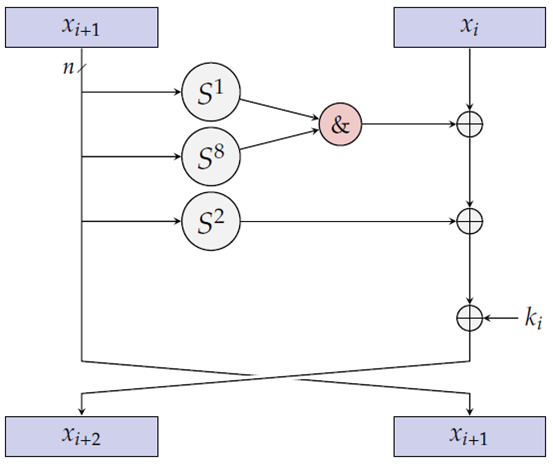
\includegraphics[width=5cm]{SIMON}
    \bicaption[fig:SIMON]{SIMON的轮函数结构}{SIMON轮函数的Feistel结构}{SIMON}{The Feistel structure of SIMON}
\end{figure}

\begin{figure}[htbp]
    \centering
    $$k_{i+m}=\begin{cases}
        c\oplus(z_j)_i\oplus k_i\oplus(I\oplus S^{-1})S^{-3}k_{i+1} & m=2\\
        c\oplus(z_j)_i\oplus k_i\oplus(I\oplus S^{-1})S^{-3}k_{i+2} & m=3\\
        c\oplus(z_j)_i\oplus k_i\oplus(I\oplus S^{-1})(S^{-3}k_{i+3}\oplus k_{i+1}) & m=4
    \end{cases}$$
    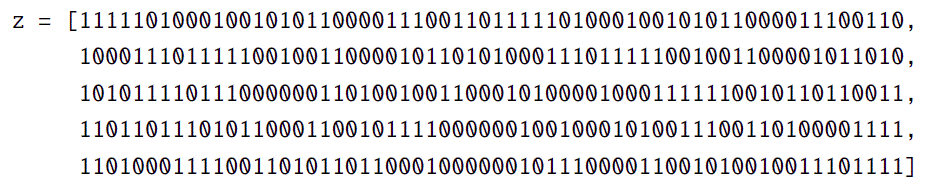
\includegraphics[width=10cm]{SIMONKey}
    \bicaption[fig:SIMONKey]{SIMON的密钥编排方案}{SIMON的密钥编排方案,其中$c$是常数,$z$是常数数组,$k_i,k_{i+1},k_{i+2}$是轮密钥,$S^j$表示循环左移$j$位,$I$表示不移位。}{SIMON}{The key schedule of SIMON, where $c$ is a constant and $z$ is a constant array, $k_i,k_{i+1},k_{i+2}$ is round keys, $S^j$ means left circular shifting by $j$ bits and $I$ means identity.}
\end{figure}

SIMON拥有很多不同的版本,有各自不同的分组长度和主密钥长度。
以最简单的分组长度32比特,密钥长度64比特,字(word)长度$n=16$比特,$m=4$为例,为了准确表示轮与轮中间状态的依赖关系,我们需要将中间状态设为$X_i=x_{i+1}||x_i$(见图\ref{fig:SIMON})。
由于SIMON的分组长度为32比特,这一点与前述的SPN结构密码无区别,但是在考虑该轮的AKI时,我们不能简单的取$X_i$中所有比特的路径中最小的AKI来计算——$X_i$和$X_{i+1}$中拥有共同的一块中间状态$x_{i+1}$,而这一块的路径必然是一样的,AKI也会相同。
因此在考虑某一轮的AKI时,我们应该事先确定好使用中间状态的某一部分。
考虑到经过一轮变换后,$X_1=x_2||x_1$,而$x_1$是明文中的一部分,因此取$x_1$作为AKI研究对象显然不合适。
因此,在考虑第$i$轮的AKI时,我们选择$X_i=x_{i+1}||x_i$中的$x_{i+1}$部分所有路径的最小AKI作为该轮的AKI。

在SIMON的密钥编排方案中,每一轮的轮密钥是由前$m$轮的轮密钥生成的。
因此,一轮轮密钥至少依赖于$mn$比特的轮密钥,则密钥依赖矩阵至少应为$\mathbb{N}^{mn\times mn}$。
在$n=16,m=4$的情况下,$k_{i+m}$依赖于$k_i,k_{i+1},k_{i+2},k_{i+3}$,因此我们设子密钥$WK_i=k_{i+3}||k_{i+2}||k_{i+1}||k_i$后,即可完整的表示出轮密钥之间的依赖关系。
可以看出这种情况下密钥依赖矩阵中,后$n$行表达出了真正的轮密钥的推导关系($k_{i+3}$的计算是由$WK_{i-1}$中的$mn$比特共同推出的),而前$(m-1)n$行中只有一个“1”(直接从上一个子密钥中搬来),只是为了保证$WK_i$中包含了足够推出$WK_{i+1}$的信息。

\begin{table}[htbp]
\centering
\begin{tabular}{c|c|c}
\hline
&\multicolumn{2}{c}{SIMON}\\
\hline
&$TKI$&$AKI$\\
\hline
$r=1$ & 1 & 1\\
$r=2$ & 4 & 4\\
$r=3$ & 10 & 10\\
$r=4$ & 20 & 20\\
$r=5$ & 34 & 34\\
$r=6$ & 50 & 50\\
$r=7$ & \textbf{64} & 63\\
$r=8$ & 64 & \textbf{64}\\
\hline
\end{tabular}
\bicaption[tab:SIMON]{SIMON的AKI}{SIMON的AKI}{AKI}{AKI of SIMON}
\end{table}

确定了两个矩阵的表示方法后,我们通过算法\ref{alg:AKI}的到SIMON的AKI,见表\ref{tab:SIMON}。
从表中可以看出,SIMON的TKI增长较慢,但前6轮都不存在密钥信息泄露,直到第7轮,密钥依赖路径的长度达到了$66>64$,但出现了3比特的密钥信息泄露,使得第7轮的AKI并没有达到理论最大值。

